\documentclass[tikz, varwidth=6in]{standalone}

\newcommand{\FA}{
  \begin{tabular}{c|c|c|c}
    \multicolumn{4}{c}{\textsc{p}}\\\hline
    \, & \, & \, & \,
  \end{tabular}
}

\newcommand{\FB}{
  \begin{tabular}{c|c|c|c}
    \multicolumn{4}{c}{\textsc{p}}\\\hline
    \(\bullet\) & \, & \, & \,
  \end{tabular}
}

\newcommand{\FC}{
  \begin{tabular}{c|c|c|c}
    \multicolumn{4}{c}{\textsc{p}}\\\hline
    \(\bullet\) & \(\bullet\) & \, & \,
  \end{tabular}
}

\newcommand{\FD}{
  \begin{tabular}{c|c|c|c}
    \multicolumn{4}{c}{\textsc{p}}\\\hline
    \(\bullet\) & \(\bullet\) & \(\bullet\) & \,
  \end{tabular}
}

% arara: pdflatex: { interaction: batchmode }
% arara: latexmk: { clean: partial }
\begin{document}
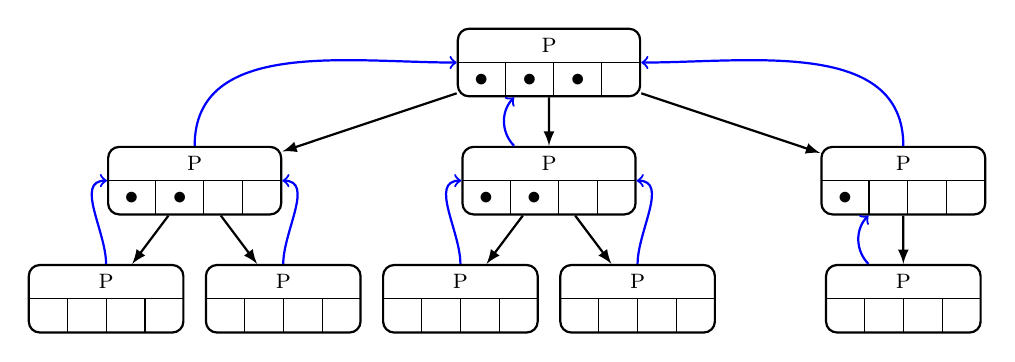
\begin{tikzpicture}[
    level distance=1.5cm,
    level 1/.style={sibling distance=4.5cm},
	level 2/.style={sibling distance=2.25cm},
    fit rounded/.style={rounded corners, draw, inner sep=+0pt},
    edge from parent/.style={draw,-latex},
    thick
]
\node[fit rounded] (T) {\FD}
	child { node[fit rounded] (TL) {\FC}
		child { node[fit rounded] (TLL) {\FA}}
		child { node[fit rounded] (TLR) {\FA}}
	}
	child { node[fit rounded] (TC) {\FC}
		child { node[fit rounded] (TCL) {\FA}}
		child { node[fit rounded] (TCR) {\FA}}
	}
	child {node[fit rounded] (TR) {\FB}
		child { node[fit rounded] (TRL) {\FA}}
	}
;
\draw[->,blue] (TL) to[out=90,in=180] (T);
\draw[->,blue] (TC) to[out=135,in=225] (T);
\draw[->,blue] (TR) to[out=90,in=0] (T);
\draw[->,blue] (TRL) to[out=135,in=225] (TR);
\draw[->,blue] (TLL) to[out=90,in=180] (TL);
\draw[->,blue] (TLR) to[out=90,in=0] (TL);
\draw[->,blue] (TCL) to[out=90,in=180] (TC);
\draw[->,blue] (TCR) to[out=90,in=0] (TC);
\end{tikzpicture}
\end{document}
